\section{What is time?}

Time is the indefinite continued progress of existence and events that occur in apparently irreversible succession from the past through the present to the future.
Time is a component quantity of various measurements used to sequence events, to compare the duration of events or the intervals between them, and to quantify rates of change of quantities in material reality or in the conscious experience.
Time is often referred to as the fourth dimension, along with the three spatial dimensions.

\section{The clock}

A clock is an instrument to measure, keep, and indicate time. The process can be either caused by a natural phenomenon or an artificial machine.

Time can be very subjective and therefore humans needed devices to measure it. In history, a large variety of devices were invented and built to measure time. While most of the early devices were meant to measure daytime, today’s clocks focus on increasing the accuracy and resolution in the deep fractions of a second.

The earliest clocks were based on the direction of sunlight, burning candles and flowing water or sand. Timekeeping based on the sun has obvious problems with weather and season change caused by axial tilt of the earth. Water clocks and hourglasses measure a fixed amount of time, like an hour, by letting water or sand fall from one reservoir into another.

Mechanical clocks were the next evolutionary step for timekeeping devices. Potential energy in form of a spring or lifted weight is used to drive a periodic cycle which is calibrated to fit a second, minute or hour. Popular examples are the pendulum clock and the wristwatch.

After tweaking the mechanical clock to be smaller and more accurate, the next step was the electrical clock. First electricity just replaced the mechanical potential energy with batteries or stationary power supply. Later, electrical circuits were used to produce periodic, high-frequency signals. The quartz crystal replaced the mechanical clock completely for the application of accurate measurements which is at least one order of magnitude more accurate.

Nowadays, atomic clocks are the most accurate clocks. They can be accurate within seconds over thousands of years. The first accurate atomic clock was based on ceasium 133 and was built in 1955. Today’s atomic clocks are based on ytterbium and form the base of the International Atomic Time (TAI).

\section{Time standards}

A time standard is a specification for measuring time. That can mean the rate at which time passes, or points in time, or both. A standard for civil time can specify time intervals as well as the time of the day.

A time standard should not be confused with a calendar. The calendar is a system of organising days. This can mean social, religious, commercial or administrative purposes. There are names for periods of time like days, weeks, months, years - where a date marks a single, specific day in this system.

The Ancient Egyptians defined a day to be 24 hours long, consisting of two 12 hour periods.

\subsection{The second}

The second is the base unit of time in the International System of Units (SI, french abbreviation for Système International d'Unités). It was originally defined as the fraction 1/86400 of the mean solar day whereas the “mean solar day” is defined by astronomical theories. Measurements showed that the rotation of Earth is not constant and has irregularities. That called for a new, more precise definition for the unit of time, leading to the SI definition that “the second is the duration of 9 192 631 770 periods of the radiation corresponding to the transition between the two hyperfine levels of the ground state of the ceasium 133 atom”.
The second may be measured by a mechanical, electrical or atomic clock.

\subsection{Greenwich Mean Time}

Greenwich Mean Time (GMT) is the mean solar time at the Royal Observatory in Greenwich. It was used as the international civil time standard until replaced by the Coordinated Universal Time (UTC). Today the term GMT is ambitious because it can mean UTC or UT1. This includes an uncertainty of up to 0.9 seconds. Because of that it should not be used for precise purposes.

\subsection{Universal Time}

Universal Time (UT) is a modern continuation of Greenwich Mean Time (GMT) and thus based on Earth’s rotation. There are several versions of it while the commonly used are Coordinated Universal Time (UTC) and UT1. All these versions except UTC are only based on Earth’s rotation. The second of UTC is also on the International Atomic Time with leap seconds added, or theoretically removed, to keep it within 0.9 seconds of UT1.

\subsubsection{Coordinated Universal Time}

Coordinated Universal Time (UTC) is world’s major time standard to regulate clocks and time. It is defined to be within 0.9 second of mean solar time at 0° longitude, the earlier GMT or today's UT1. The term UTC is often mixed with GMT, which is no longer precisely defined by the scientific community.

\subsubsection{Leap second}

\begin{figure}[tb]
	\centering
	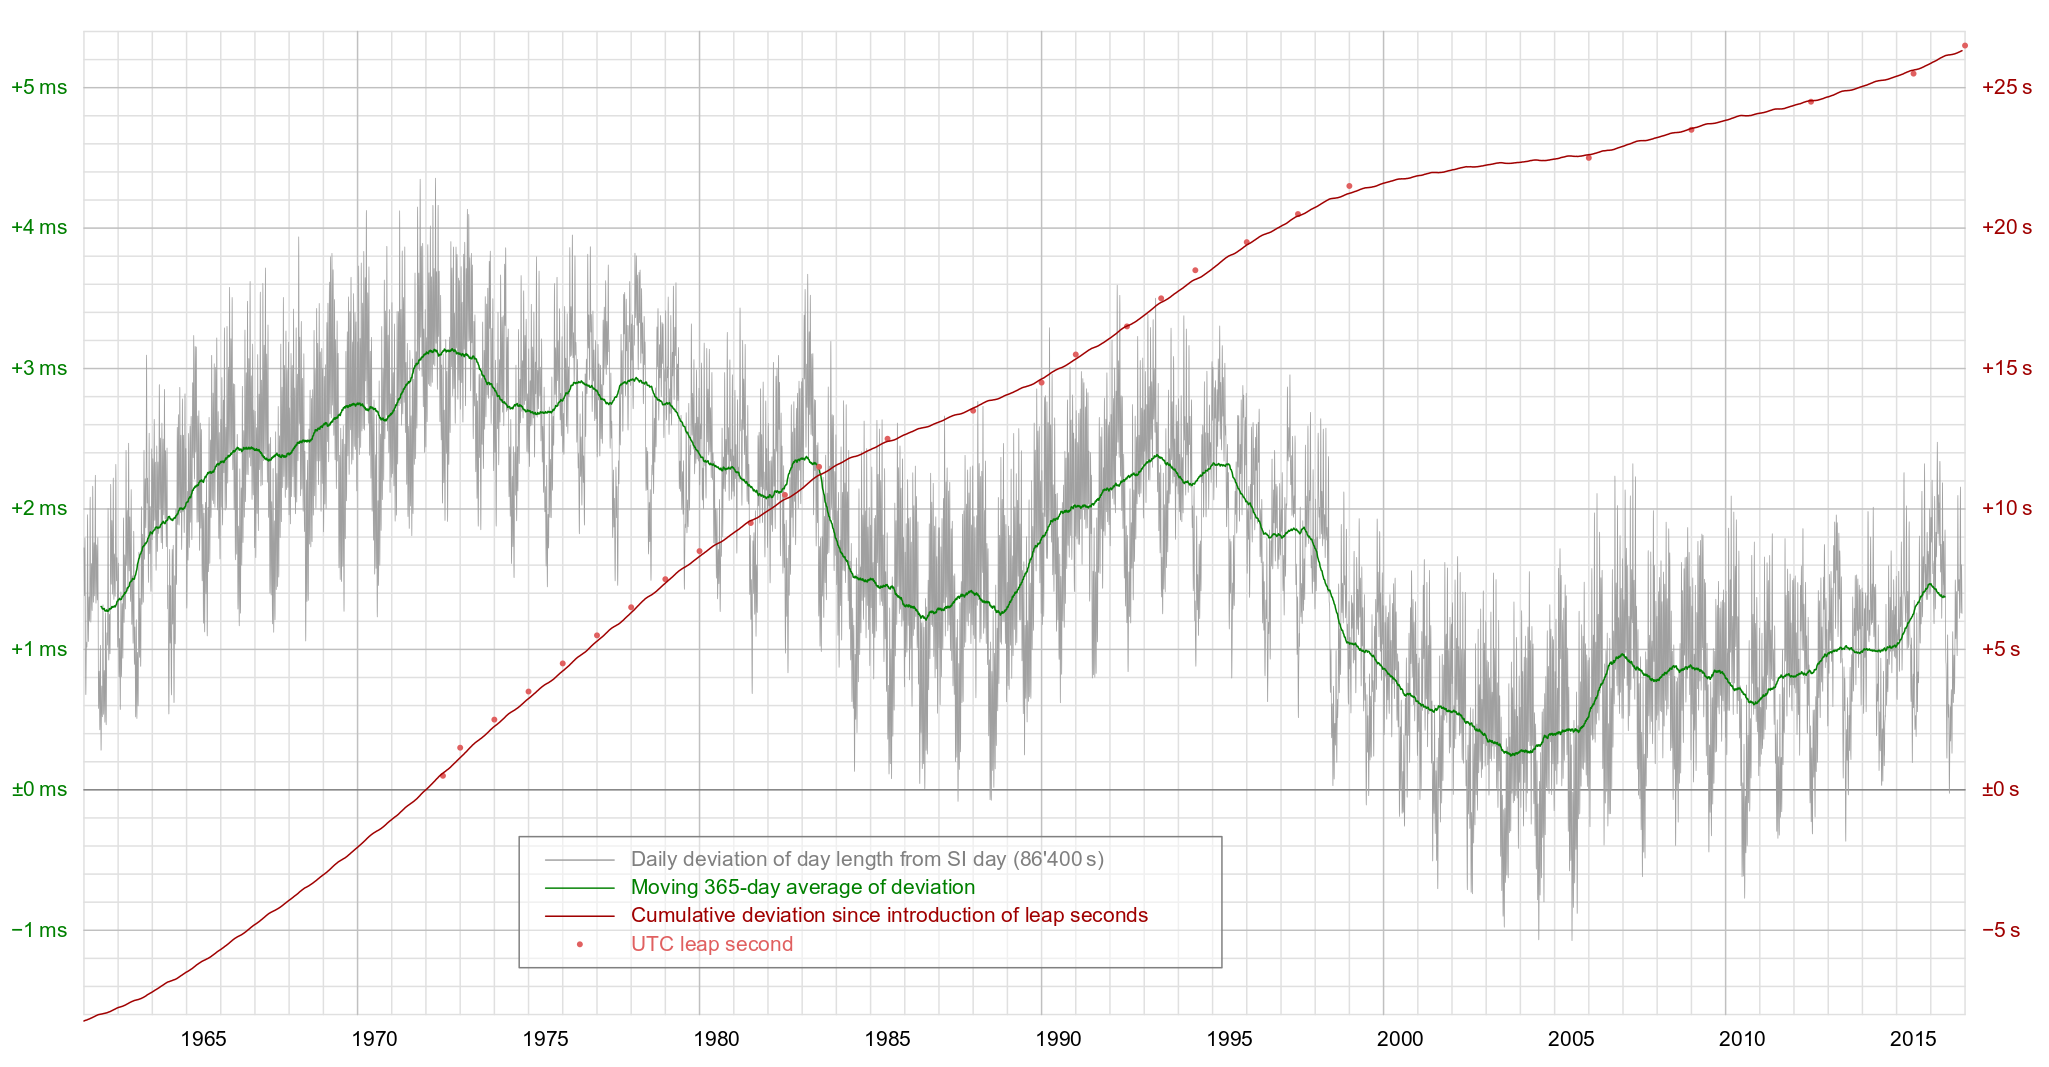
\includegraphics[width=1.0\textwidth]{figures/leap_second.png}
	\caption{Deviation of day length from SI day}
	\label{fig:leap_second}
	% https://upload.wikimedia.org/wikipedia/commons/5/5b/Deviation_of_day_length_from_SI_day.svg
\end{figure}

A leap second is a one-second adjustment that is occasionally applied to Coordinated Universal Time (UTC) to keep the difference with the mean solar time, UT1, within 0.9 second. Without such a correction UTC would drift away from UT1 caused by irregularities of Earth’s rotation rate. Since this concept was implemented in 1972 there were 27 leap seconds added with the most recent one on December 31, 2016 at 23:59:60 UTC.

In figure \ref{fig:leap_second} we can see the deviation of day length from SI day, the moving average, the cumulative deviation and the applied leap seconds.

\subsection{International Atomic Time}

The International Atomic Time (TAI, French abbreviation for Temps Atomique International) is a high-precision atomic coordinate time standard which is based on the notional passage of proper time on Earth’s geoid. It is the basis for Coordinated Universal Time (UTC). TAI can only differ from UTC by a multiple of a full second as a result of the definition of UTC.

